% Basic LaTeX template for NE 204 lab report
%defines the type of document you will be using
%Most journals have their own style.
\documentclass[11pt]{article}

%==============================================================================
%%% Everything between the "="'s is the preamble.
%%% Define packages and meta data here

% Common packages
\usepackage{amsmath}    % Expanded math
\usepackage{amssymb}    % Expanded math symbols
\usepackage{graphicx}   % For images
\usepackage[most]{tcolorbox}
%mhchem is beneficial for Nuke Eng.
\usepackage[version=3]{mhchem} % For nuclide formatting
\usepackage{float}

% All images/figures will be stored in the images folder.
% Specify that here so pdflatex knows where to look for images.
\graphicspath{{./images/}}

% Metadata
\title{Lab 0 - Linear Calibration of a High Purity Germanium Detector}
\author{Matthew Marshall}
\date{\today}
%==============================================================================

\begin{document}

% Compile metadata from preamble into a nicely-rendered title section
\maketitle

% The *'s next so section/subsection definitions suppresses numbering
% \section*{Introduction}
% The *'s next so section/subsection definitions suppresses numbering
\section*{Abstract}
\label{sec:abstract}
This report details the importance and process of generating a two-point
energy calibration using $^{137}$Cs and $^{241}$Am to produce a calibrated
$^{133}$Ba.


\section{Introduction}
\label{sec:intro}
The purpose of Lab 0 was to perform a two-point linear calibration between two gamma-ray photopeaks.
In gamma-ray spectroscopy, determining which gamma-rays are present is an important aspect of
radiation detection, and relying solely on the raw channel output makes it difficult to determine the gamma-ray energies
present. By performing an energy calibration, a relationship is formed between peak channel position
and the associated gamma-ray energy \cite{gilmore}. This relationship helps with the identification and discernment of
gamma-ray photopeaks from noise or spurious results, which has an
importance for non-proliferation reasons. Thus, having
a properly calibrated spectrum is an essential component of gamma-ray spectroscopy.
The following report details the process and results of a two-point linear calibration using $^{137}$Cs and $^{241}$Am as
calibration sources.


\section{Methods}
\label{sec:meth}
The data for this lab came from a HPGe detector collected by Dr. Ross Barnowski.
The sources used to generate the spectrum are shown in Table \ref{table:source}.
\vspace{15mm} %5mm vertical space
\begin{table}[H]
  \begin{center}
    \begin{tabular}{|c|}
      \textbf{Source}\\
      \hline
      $^{241}$Am\\
      $^{133}$Ba\\
      $^{60}$Co\\
      $^{137}$Cs\\
      $^{152}$Eu\\
      \hline
    \end{tabular}
    \caption{Gamma-ray lines used in the calibration}
    \label{table:source}
  \end{center}
\end{table}

The energy calibration was performed using a two-point linear fit between
$^{137}$Cs and $^{241}$Am. To perform the calibration, a python program searched
the raw spectrum data of $^{137}$Cs and $^{241}$Am looking for
the largest peaks within the spectrum. The program iterated over the spectrum for the
number of gamma-ray energies present since there should only be peaks corresponding
to the number of gamma-ray energies present. Before the program iterated over the raw spectrum,
the data needed to be "cleaned". Noise from the detector could obscure some of the peaks
found from iterating peak heights. With a peak found, the centroid of the peak was
recorded, and subsequently, utilizing a pre-defined width that incapsulates
the whole peak, the program fit a Gaussian and a linear model to this portion of the data.

After modeling the data with the Gaussian and linear model, the peak was
set to zero so during the next iteration the same peak is not found again.
The width of the peak was determined from first analyzing the spectrum and establishing
the average width of each peak.

Once all of the peaks were discovered, polyfit within python was used to
plot a linear line. The inputs for polyfit were the position of the peak and
the actual gamma-ray energies. The slope-intercept from polyfit was applied
to the channel numbers within the $^{133}$Ba spectrum. Finally, to plot the data
I did the newly calibrated channel numbers vs the original $^{133}$Ba spectrum.


\section{Results}
\label{sec:res}
The raw spectrum of $^{133}$Ba is depicted in Figure \ref{fig:raw_data}.

\begin{figure}[H]
\centering
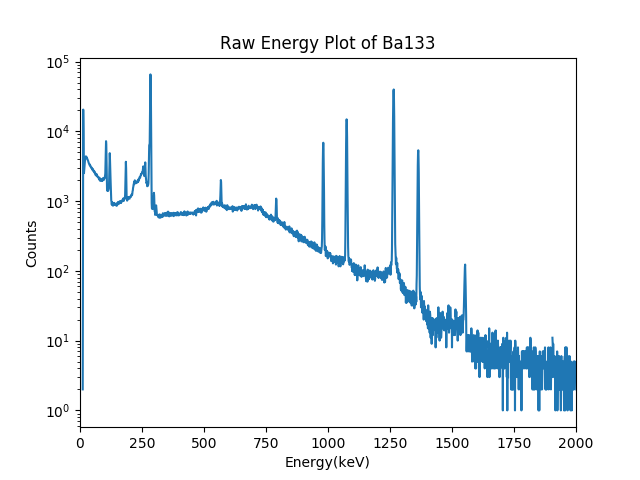
\includegraphics[scale=0.8]{images/Raw_spectrum.png}
\caption{Raw data of $^{133}$Ba produced from a HPGe detector.}
\label{fig:raw_data}
\end{figure}

Inspection of Figure \ref{fig:raw_data} shows that the data has not been calibrated yet.
For this analysis, I used 5 peaks from $^{133}$Ba
detailed in \ref{table:energy} \cite{Untitled27:online}.

\begin{table}[H]
\caption{$^{133}$Ba Gamma-ray Energies}
\begin{center}
\begin{tabular}{|l|c|c|r|}
\textbf{Source} & \textbf{Energy (keV)}\\
\hline
$^{133}$Ba    &  80.9979 \\
              &  276.3989 \\
              & 302.8508  \\
              & 356.0129 \\
              & 383.8485 \\
\hline
\end{tabular}
\end{center}
\label{table:energy}
\end{table}

I excluded 79.6142 keV from the energy list because it blurs together with
80.99 keV into one photopeak due to the energy resolution
of the HPGe. A better resolution detector would be needed to distinguish
these two peaks. Thus, I removed it so the iterator in the program will
not search for a peak that is not present.

After performing the linear calibration with $^{137}$Cs and $^{241}$Am,
a slope-intercept was found.
\vspace{5mm} %5mm vertical space
\begin{equation}
E = 0.28054*x + 1.26023
\end{equation}
\vspace{5mm} %5mm vertical space

The slope and intercept was applied to the channel number of the raw Ba133 data.
Figure \ref{fig:CE} depicts the two-point calibration.

\begin{figure}[H]
\centering
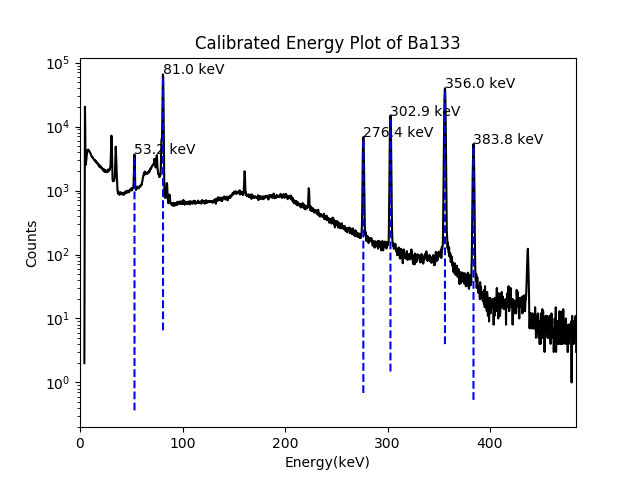
\includegraphics[scale=0.8]{images/Ba133_calibrated.png}
\caption{Calibrated $^{133}$Ba data with their corresponding gamma-ray energies
depicted by dashed blue lines}
\label{fig:CE}
\end{figure}

The difference between the calibrated peak locations and the expected peak
are shown in Table \ref{table:difference}.

\begin{table}[H]
\caption{$^{133}$Ba Gamma-ray Energies}
\begin{center}
\begin{tabular}{|l|c|c|r|}
\textbf{Source} & \textbf{Energy (keV)} & \textbf{Calibrated Energy} & \textbf{Difference (\%)}\\
\hline
$^{133}$Ba    &  80.9979 +/- 0.0011  & 81.0231 +/- 0.02546 & 0.03108 +/- 0.03147 \\
              &  276.3989 +/- 0.0012 & 276.4462 +/- 0.0053907 & 0.017148 +/- 0.001998 \\
              & 302.8508 +/- 0.0005 & 302.8877 +/- 0.008467 & 0.01217 +/- 0.0028006  \\
              & 356.0129 +/- 0.0007 & 356.038 +/- 0.006710 & 0.0070492 +/- 0.001895 \\
              & 383.8485 +/- 0.0012 & 383.8706 +/- 0.009235 & 0.005751 +/- 0.0024263 \\
\hline
\end{tabular}
\end{center}
\label{table:difference}
\end{table}

Based on Table \ref{table:difference}, the percent difference between the actual peak energies
and the calibrated spectrum is minute, which would be expected since semiconductors are nearly
linear with energy.


\section{Discussion}
\label{sec:disc}
The two-point energy calibration proved to be an effective method to calibrate a
spectrum. After cleaning the raw data to remove electronic noise and excluding
the 79 keV line for $^{133}$Ba, the calibrated data corresponded well with the actual
gamma-ray energies. There was a small amount of error between the gamma energies
and the photopeaks, but this is expected because I only used a two-point
energy calibration. Once more sources are added in to the calibration that span the
entire energy range, the photopeaks
should correspond better with their corresponding energies.


% Bibliography
\bibliographystyle{unsrt}
% Refers to a bibtex file in the current dir named "references.bib"
\bibliography{references}

\end{document}
